%\newcommand{\CLASSINPUTbaselinestretch}{1.0} % baselinestretch
%\newcommand{\CLASSINPUTinnersidemargin}{1in} % inner side margin
%\newcommand{\CLASSINPUToutersidemargin}{1in} % outer side margin
%\newcommand{\CLASSINPUTtoptextmargin}{1in}   % top text margin
%\newcommand{\CLASSINPUTbottomtextmargin}{1in}% bottom text margin

\documentclass[journal,a4paper]{IEEEtran}


\usepackage[pdftex]{graphicx}  
\usepackage[cmex10]{amsmath}

\usepackage{float}
%maakt caption van figuren groter
\usepackage{caption}
\usepackage{amsmath}
\usepackage{epstopdf}
\usepackage{textcomp}
\usepackage{gensymb}
\usepackage[titlenumbered,algoruled, linesnumbered]{algorithm2e}
\usepackage{booktabs}
\usepackage[T1]{fontenc}
\usepackage[utf8]{inputenc}
\usepackage{hyperref}


\newcommand\MYhyperrefoptions{bookmarks=true,bookmarksnumbered=true,
pdfpagemode={UseOutlines},plainpages=false,pdfpagelabels=true,
colorlinks=true,linkcolor={black},citecolor={black},pagecolor={black},
urlcolor={black},
pdftitle={Flip the virus:\\ A gametheoretic approach to cybersecurity},
pdfauthor={Sophie Marien}}

\begin{document}

\title{Flip the virus:\\ A gametheoretic approach to cybersecurity}
\author{Sophie Marien\\
DistriNet KULeuven \\
sophie.m.marien@gmail.com}
\maketitle

\IEEEcompsoctitleabstractindextext{%
\begin{abstract}
Recently, high profile targeted attacks such as the attack on Belgacom (a major Belgian telcom), have demonstrated that even the most secure
companies can still be compromised, and that moreover such attacks can go undetected for a while. 
FlipIt has been proposed by a group of
researchers at RSA to model such stealthy takeovers. It is a 2-players game composed of a single
attacker, a single defender and a single shared resource. The
players will try to gain control over the shared resource and they
do this in a stealthy way. FlipIt does however not take into account that a move may not be instantaneous, but has a certain delay. In this paper we adapt FlipIt
such that we can use it to model the game of defending a
company network that is attacked by a virus. The FlipIt formulas
are adapted such as to take the delay for virus propagation into account. 
\end{abstract}
}

\IEEEdisplaynotcompsoctitleabstractindextext
\IEEEpeerreviewmaketitle


\section{Introduction}
\label{sec:inleiding}
\IEEEPARstart{I}{n this era} where digitalization becomes prominent in every aspect of our lives, where technology is growing fast and where businesses are always under attack, security becomes an issue of increasing complexity. Without security, there is no protection to keep somebody out of a system. It is the same as leaving the door of your house wide open for everyone to come in. \\

Why is it so important to keep a system secure?  Many businesses store confidential information on clients, which can be lost and possible be abused by competitors through data leakage. Also, disruption caused by DDoS attacks, may results in businesses failing to meet their service-level agreements. Ultimately, system and network security helps protecting a business's reputation, which is one of its most important assets. \\
% A hacker will be a person that seeks exploits or weaknesses in a system or network in order to gain access.  Many of those attacks have a different cause. Some of the attacks by a hacker can be benign, others can be harmful. There are various ways to break into a system. Viruses, worms, spyware and other malware are the number two of the top external threats that a business faces, according to the security report kaspersky 2014 \cite{kaspersky} (number one is Spam). Furthermore these kind of threats also causes the greatest percentage in loss of data. These threats will infect the network by means of a virus that will propagate through the network.  Most of the attacks are Advanced Persistent Threats (APT). \\
 

A particular kind of frequently occurring threats are Advanced Persistent Threats (APT). An APT is a targeted cyber attack that targets organisations in a stealthy way and that can stay undetected for a long period. This makes it so hard to protect a network or a system against an APT. Bruce Schneier describes an APT as something different and stronger than a conventional threat: ''\textit{A conventional hacker or criminal isn't interested in any particular target. He wants a thousand credit card numbers for fraud, or to break into an account and turn it into a zombie, or whatever. Security against this sort of attacker is relative; as long as you're more secure than almost everyone else, the attackers will go after other people, not you. An APT is different; it's an attacker who - for whatever reason - wants to attack you. Against this sort of attacker, the absolute level of your security is what's important. It doesn't matter how secure you are compared to your peers; all that matters is whether you're secure enough to keep him out}'' - Bruce Schneier \cite{APTBruce}.\\

Since it is so difficult to protect a system or a network against APT's, researchers have been looking for effective ways to predict in advance which defence strategy might be the better one. 
Game theory is gaining increasing interest as an effective technique to model and study Cyber Security. Game theory analyses the security problem as a game where the players are an attacker and a defender of a system, and where both players have to make decisions. In particular, both players will aim for the strategy that results in a maximal benefit for them.  Researchers at RSA made a game theoretic framework to model targeted attacks. They study the specific scenario where a system or network is repeatedly taken over completely by an attacker and this attack is not immediately detected by the defender of the system or network. In game theory, such a game is known as ''FlipIt'' \cite{FlipIt}. This is a two players game where the attacker and the defender are competing to get control over a shared resource. Both players do not know who is currently in control of the resource until they move. In FlipIt every move gives them immediately control over the resource. But what if the attacker moves and it takes a while before the attacker gets full control over the resource? FlipIt does not take into account that a move may not be instantaneous, but has a certain delay. Consider for example a network with different nodes ( laptops, datacenters) as a resource. The attacker drops a virus on one of the nodes and then wait till this virus infects the whole network. The attacker will only be in control of the resource once the whole network is infected. \\

This paper proposes the adaptation of the FlipIt formulas as presented in \cite{FlipIt} such as to take the delay for virus propagation into account. In the next section we first present the original FlipIt game. Then section \ref{ch:flipitvirus} presents the FlipIt game with virus propagation. Section \ref{ch:extendedWork} presents some related work. Section \ref{ch:conclusion} concludes the paper and presents avenues for further research.

\section{The FlipIt game}
\label{ch:FlipItGame}
FlipIt is a game introduced by van Dijk et al. To understand how to model a FlipIt game with virus propagation it is important to get familiar with the concepts of the normal FlipIt game and its notations.  Therefore, we first explain the framework of FlipIt and introduce the most important formulas that will be used throughout the paper. \\

FlipIt is a two-players game with a shared single resource that the players want to control as long as possible. The shared resource can be a password, a network or a secret key depending on the setting being modelled. In the remainder of the paper we name the two players the attacker, denoted by the subscript \textit{A} and the defender, denoted by subscript \textit{D}. 

The game begins at $t=0$ and continues indefinitely ($t \rightarrow \infty $). The time in the game is assumed as being continuous, but a discrete time could also be considered. To get control over the resource, the players $i$, with $i \in \{A,D\}$, can flip the resource at any given time. A flip will be regarded as a move from a player \textit{i}. Each move will imply a certain cost $k_{i}$ and the cost can vary for each player. Both players will try to minimize their cost. Adding a cost will prevent players to move too frequently. \\

The unique feature of FlipIt is that every move will happen in a stealthy way, meaning that the player has no clue that the other player (his adversary) has flipped the resource. For instance, the defender will not find out if the resource has already been compromised by the attacker until he flips the resource himself. The goal of the player is to maximize the time that he or she has control over the resource while minimizing the total cost of the moves. A move can also result in a "wasted move", called a flop. It may happen that the resource was already under control by the player. If the player moves when he or she has already control over the resource, he or she would have wasted a move since it does not result in a change of ownership, so the cost is wasted. \\


\begin{figure}[hbtp]
\centering
\includegraphics[scale=0.5]{../../doc/template/Images/DefFlipit}
\caption{A representation of a FlipIt game where both players are playing periodically and at discrete time intervals. Every move or flip is indicated by a blue or orange circle. The attacker is represented in orange and plays with a period of $\delta_{A}=4$. The defender is represented in blue and plays with a period of $\delta_{D}=3$. The blue and orange rectangles represent the amount of time the respective player is in control of the resource.}
\label{fig:FLipItDefault}
\end{figure}



The state of the resource is denoted as a time-dependent variable $C=C_{i}(t)$. 
$C_{D}(t)$ is 1 if the game is under control by the defender and 0 if the game is under control by the attacker. Reversely, $C_{A}(t)$ will be 1 if the game is under control by the attacker and 0 if under control by the defender. So, $C_{A}(t)= 1 - C_{D}(t)$.
The game starts with the defender being in control: $C_{D}(0)= 1$. \\


The players receive a benefit equal to the time units they were in possession of the resource minus the cost of making their moves. The cost of a player \textit{i} is denoted by $k_{i}$. 
The total gain of player \textit{i} is equal to the total amount of time that a player \textit{i} has owned the resource from the beginning of the game up to time \textit{t}. It is expressed as follows:
\begin{equation}\label{first}
G_{i}(t) = \int_0^t \! C_{i}(x) dx.
\end{equation}
If we add up the gain of the defender and the gain of the attacker it should sum up to t:
\begin{equation}\label{first}
G_{D}(t) + G_{A}(t) = t
\end{equation}
The average gain rate of player \textit{i} is defined as:
\begin{equation}\label{first}
\gamma_{i}(t) = G_{i}(t)/t.
\end{equation}
And thus for all $t > 0$ :
\begin{equation}\label{first}
\gamma_{D}(t) + \gamma_{A}(t) = 1
\end{equation}
Let $\beta_{i}(t)$ denote player's \textit{i} average benefit upto time \textit{t}:
\begin{equation}\label{first}
\beta_{i}(t) = \gamma_{i}(t) - k_{i}\alpha_{i}.
\end{equation}
This is equal to the fraction of time the resource has been owned by player \textit{i}, minus the cost of making the moves. ~$ \alpha_{i}$ defines the average move rate by player \textit{i} up to time \textit{t}.
In a given game, the asymptotic benefit rate (or simply benefit) will be defined as the lim inf of the average benefit because time t will increase to infinity and the average benefit may not have limiting values.
\begin{equation}
\beta_{i}(t)  = \lim_{t \to \infty} inf \beta_{i}(t) 
\end{equation}
\\


\subsubsection{strategies}
Because the players move in a stealthy way, there are different types of feedback that a player can get while moving. These types of feedback can be divided into two groups of strategies. The non-adaptive strategies and the adaptive strategies. These are described in table \ref{table:Strategies}. \\

If there is no feedback for neither of the players, we have a non-adaptive strategy. Because a player does not receive any feedback during the game he will play in the same manner against every opponent. The strategy is called non-adaptive because the playing strategy is not dependent on the opponents movements. An interesting subclass of the non-adaptive strategies is the one where the time intervals between two consecutive moves are generated by a renewal process. An example of such renewal strategy is the periodic strategy where the time between two consecutive moves of the players are a fixed interval. An exponential strategy is a renewal strategy in which the interval between two consecutive moves is exponentially distributed. \\
In case there is feedback, a player can adapt his strategy to the information received about the opponent's moves. Depending on the amount of information received, two subclasses of adaptive strategies can be identified. The Last Move (LM) strategies represent the class where whenever a player flips he will find out the exact time that the opponent played the last time. In the second class, called Full History (FH), whenever a player flips he will find out the whole history of the opponent's move. \\
In this paper we will focus on the non-adaptive strategies. This choice is motivated by the fact that in a security game a player (defender or attacker) rarely has information about the moves (last move or full history) of his opponent.  \\


 \begin{table}
 \centering
 \begin{tabular}{ l | c  }
  \textbf{Categories} & \textbf{Classes of Strategies} \\
  \hline Non-adaptive (NA) & Renewal \\
  & - Periodic \\
  & ~~~ - Exponential \\
  & General non-adaptive \\
  \hline Adaptive (AD) & Last move (LM) \\
  & Full History (FH) \\  
\end{tabular}
 \caption{Hierarchy of Classes of strategies in FlipIt}
 \label{table:Strategies}
 \end{table}


The study of the different strategies by means of FlipIt framework allows to derive a number of interesting results:  
\begin{itemize}
\item periodic games dominate the other renewal strategies, meaning that it is always advantageous to play periodically against an opponent with a renewal strategy;
\item periodic games are disadvantageous against players following a Last Move adaptive strategy;
\item if the defender plays with a periodic rate that is fast enough he'll force the attacker to drop out;
\item any amount of feedback about the opponent received during the game, benefits to a player.
\end{itemize}
 

\section{FlipIt with virus propagation}
\label{ch:flipitvirus}
A FlipIt game consists of a single resource. To represent the security problem, the game now defines its single resource as a computer network with multiple
nodes. One of the players, the defender, will try to defend his network. The defender
will do this by flipping all the nodes of the network (i.e. the entire resource) in every move he plays. The
attacker, the other player, will try to infect all the nodes in the network. The attacker
will do this by flipping the node in the graph that can infect all the nodes in the
shortest possible time. After dropping a virus on the first node, it takes a while for the virus to infect the entire network. Since the original FlipIt game works with a single resource that is always flipped entirely, the assumption is made that the attacker is considered to gain immediate full control over the resource when the network has been infected, even it is only one node that has been infected.\\

In reality however, after dropping a virus on the first node, it takes a while for the virus to infect
the entire network. So, the assumption that the attacker has full control over the resource as soon as a node has been infected, is not realistic. The attacker has only control of the network once all or a sufficient number of nodes are infected. 
The time that it takes for the virus to infect every node (or a sufficient number of nodes) will be
denoted as an infection-delay variable \textit{d} (called 'delay' for short in the remainder of this paper). If we want to measure how long it takes for the virus to
infect all the nodes in the network, we have to calculate the shortest path from the
first infected node to the farthest node. Rather than denoting the time needed for infecting \textit{all} the nodes, the variable $d$ can also be used to denote the time needed to infect \textit{a sufficient number} of nodes.

Assume that an attacker attacks at time \textit{t}, he doesn't get immediate control over the resource, but he only gains control at time \textit{t + d}, with $d$ denoting the time needed to infect a sufficiently number (or all) nodes. If the defender flips the network before the period $d$ has elapsed (so, somewhere between $t$ and $t + d$), then the attacker will never gain full control over the resource. This implies that the mathematical formulas for gain and benefit need to be adapted to the fact that the attacker loses part of its benefit because of this delay. In the remainder of this paper, we will adapt the formalization of the FlipIt game using the variable $d$. \\

The formalization starts from the model of the non-adaptive continuous basic FlipIt game where players use a periodic strategy with a random phase. This choice is motivated by the assumption that in most organisations, the defence strategy is to periodically defend the network. This corresponds to a periodic defender strategy.  A periodic attacker strategy is assumed as well, to be able to compare the results with the periodic strategy of the FlipIt game in \cite{FlipIt}. %, as this also corresponds to a common real life strategy. %nog eventueel verder te motiveren
Further research can investigate the effect of relaxing this assumption. \\

Similarly as in \cite{FlipIt}, we split the formalization in two cases. The first case is where the defender plays at least as fast as the attacker, the second case is where the attacker plays at least as fast as the defender. For each of these cases, first the benefit formula of the basic case without delay is presented, and then the delay is introduced.  \\

\subsection{Formalization the benefit formula including the infection-delay}
 A Periodic strategy is a non-adaptive renewal strategy where the time intervals between consecutive moves are a fixed period, denoted by $\delta$. Moreover it has a random phase, that is chosen uniformly and random in the interval $[0,\delta]$ for the first move. The average rate of play of a player is denoted by $\alpha_{i} = \dfrac{1}{\delta_{i}}$. \\
~~\\

\subsection*{\textbf{Case 1:} $\delta_{D} \leq \delta_{A} $ (The defender plays at least as fast as the attacker.) }

Let $r = \dfrac{\delta_{D}}{ \delta_{A} }$. The intervals between two consecutive defender's moves have length $\delta_{D}$. Consider a given defender move interval. The probability over the attacker's phase selection that the attacker moves in this interval is r. Given that the attacker moves within the interval, he moves exactly once within the interval (since $\delta_{D} \leq \delta_{A} $) and his move is distributed uniformly at random. \\

The expected period of attacker control within the interval would be r/2, without considering the delay by a virus. Therefore the benefit for the attacker, without considering the delay, can be expressed as follows:

\begin{equation}\label{first}
\beta_{A}(\alpha_{D},\alpha_{A}) =\dfrac {r} {2} - k_{A} \alpha_{A} = \dfrac {\delta_{D}} {2\delta_{A}} - k_{A} \alpha_{A}  
\end{equation}\\

Correspondingly, the benefit for the defender can be expressed as:
\begin{equation}\label{first}
\beta_{D}(\alpha_{D},\alpha_{A}) =1 -  \dfrac {r} {2} - k_{D} \alpha_{D} = 1 - \dfrac {\delta_{D}} {2\delta_{A}} - k_{D} \alpha_{D} 
\end{equation}

\begin{figure}[hbtp]
\caption{The first FlipIt game is one without virus propagation. The second one is with virus propagation and \textit{d} = 1. The delay is denoted with an arrow.}
\centering
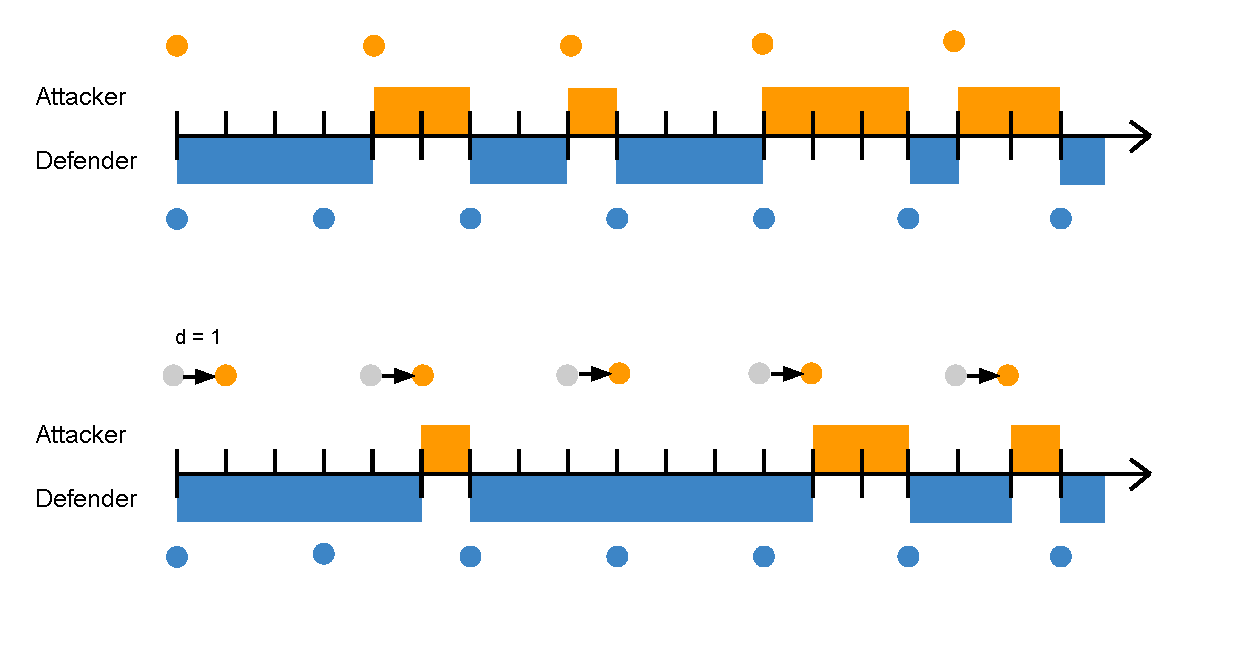
\includegraphics[scale=0.4]{../../doc/template/Images/FLipItCase1.pdf}
\label{fig:delaycase1}
\end{figure}


However, because of the delay required for virus propagation, the maximal time of control is reduced to $\delta_{D}-d$ , see figure \ref{fig:delaycase1}. There is a probability of \textit{r} that the attacker will move in the interval of the defender. However, the gain will not be half of the interval. Indeed, the attacker has to play soon enough to gain control, meaning that the attacker has to play during the period of $\delta_{D}-d$ during the interval of the defender. The probability that the attacker plays soon enough is $\dfrac{\delta_{D}-d}{\delta_{D}}$ and this will give the attacker an average gain of $\dfrac{\delta_{D}-d}{2}$. If the attacker moves after the period of $\delta_{D}-d$, the gain of the attacker will be zero. The probability that this happens is  $\dfrac{d}{\delta_{D}}$. The average gain rate of the attacker can then be expressed as follows if we look at one interval of the defender:
\begin{equation}\label{first}
\gamma_{A}(\alpha_{D},\alpha_{A}) = \dfrac {1}{\delta_{D}} [ \dfrac{\delta_{D}}{\delta_{A}} \cdot \dfrac{\delta_{D}-d}{\delta_{D}} \cdot \dfrac{\delta_{D}-d}{2} + \dfrac{\delta_{D}}{\delta_{A}} \cdot \dfrac{d}{\delta_{D}} \cdot 0 ]
\end{equation}

To derive the benefit, the cost of moving is subtracted from the average gain. 
\begin{equation}\label{first}
\beta_{A}(\alpha_{D},\alpha_{A}) = \dfrac { (\delta_{D}-d) ^{2}} {2 \cdot \delta_{D}  \delta_{A}} - k_{A} \alpha_{A}
\end{equation}
\begin{equation}\label{first}
\beta_{A}(\alpha_{D},\alpha_{A}) = \dfrac { \delta_{D}} {2 \cdot \delta_{A}} - k_{A} \alpha_{A} - ( \dfrac{d^{2}}{2 \cdot \delta_{A} \delta_{D}} - \dfrac{d}{\delta_{A}} )
\end{equation}
 
 
 The benefit of the defender is expressed as follows:
 \begin{equation}\label{first}
\beta_{D}(\alpha_{D},\alpha_{A}) = 1 - \dfrac { (\delta_{D}-d) ^{2}} {2 \cdot \delta_{D}  \delta_{A}} - k_{D} \alpha_{D}
\end{equation}
~~\\
We can easily see that when $d$=0, we obtain the formula of the original FlipIt game.\\


\subsection*{\textbf{Case 2:} $\delta_{A} \leq \delta_{D} $ (The attacker plays at least as fast as the defender.) }

First let $r = \dfrac{\delta_{D}}{ \delta_{A} }$. The intervals between two consecutive attacker's moves have length $\delta_{A}$. Consider a given attackers move interval. The probability over the attacker's phase selection that the defender moves in this interval is $\dfrac{\delta_{A}}{ \delta_{D} } = (1/r)$. Given that the defender moves within the interval of the attacker, he moves exactly once within this interval (since $\delta_{A} \leq \delta_{D} $) and his move is distributed uniformly at random. \\

A similar analysis as in case 1 for a FlipIt game without virus propagation yields the following benefits:

\begin{equation}\label{first}
\beta_{D}(\alpha_{D},\alpha_{A}) = \dfrac {1} {2r} - k_{D} \alpha_{D} = \dfrac {\delta_{A}} {2\delta_{D}} - k_{D} \alpha_{D} 
\end{equation}
\begin{equation}\label{first}
\beta_{A}(\alpha_{D},\alpha_{A}) =1 - \dfrac {1} {2r} - k_{A} \alpha_{A} = 1- \dfrac {\delta_{A}} {2\delta_{D}} - k_{A} \alpha_{A}  
\end{equation}\\


For the case with a virus we consider two cases, Case a and Case b, depending on whether the delay is shorter or longer than the difference between the attacker's and the defender's period.  \\


\subsubsection*{\textbf{Case a:} $d + \delta_{A} \leq \delta_{D}$}
~~\\
Consider a timespan $\delta_{A} + d$, representing the attacker's interval followed by the delay period in his next interval. The defender will never move twice during this timespan because $\delta_{A} + d \leq \delta_{D}$. The defender will move during the interval of the attacker with a probability of $\dfrac{\delta_{A}}{\delta_{D}} $. When this happens the defender will end with being in control at the end of the interval. In the next interval the attacker will have to regain control, meaning that during the delay, the defender stays in control, see figure \ref{fig:case2} cases (1) and (2). This means that the defender will keep the control over the resource in the next interval over a period of the delay, namely \textit{d}. Because $d + \delta_{A} \leq \delta_{D}$ the next move of the defender in this second interval will never occur during the delay, meaning that the entire delay can be considered as an extra benefit resulting of a play in the previous interval. 
So, every time the defender plays, he will get an average gain of $\dfrac{\delta_{A}}{2}$ in the interval where he plays and in the next interval will always receive a extra gain of $d$, yielding a total average gain per interval of
$\dfrac{(d+\dfrac{\delta_{A}}{2})}{\delta_{A}}$

The total gain  rate of the defender is then the probability that the defender will move during an interval of the attacker multiplied by the total average gain per interval: 

\begin{equation}\label{first}
\gamma_{D}(\alpha_{D},\alpha_{A}) = \dfrac{\delta_{A}}{\delta_{D}} \cdot \dfrac{(d+\dfrac{\delta_{A}}{2})}{\delta_{A}} 
\end{equation}
\begin{equation}\label{first}
\gamma_{D}(\alpha_{D},\alpha_{A}) = \dfrac{\delta_{A}}{2\delta_{D}} + \dfrac{d}{\delta_{D}} 
\end{equation}\\
This yields in the following benefit formula:
\begin{equation}\label{first}
\beta_{D}(\alpha_{D},\alpha_{A}) = \dfrac{\delta_{A}}{2\delta_{D}} + \dfrac{d}{\delta_{D}} - k_{D} \alpha_{D} 
\end{equation}\\

The benefit for the attacker will be as follows:
\begin{equation}\label{first}
\beta_{A}(\alpha_{D},\alpha_{A}) = 1 -\dfrac{\delta_{A}}{2\delta_{D}} - \dfrac{d}{\delta_{D}} - k_{A} \alpha_{A} 
\end{equation}\\

\begin{figure}[hbtp]
\caption{Case 2 where d + deltaA < deltaD}
\centering
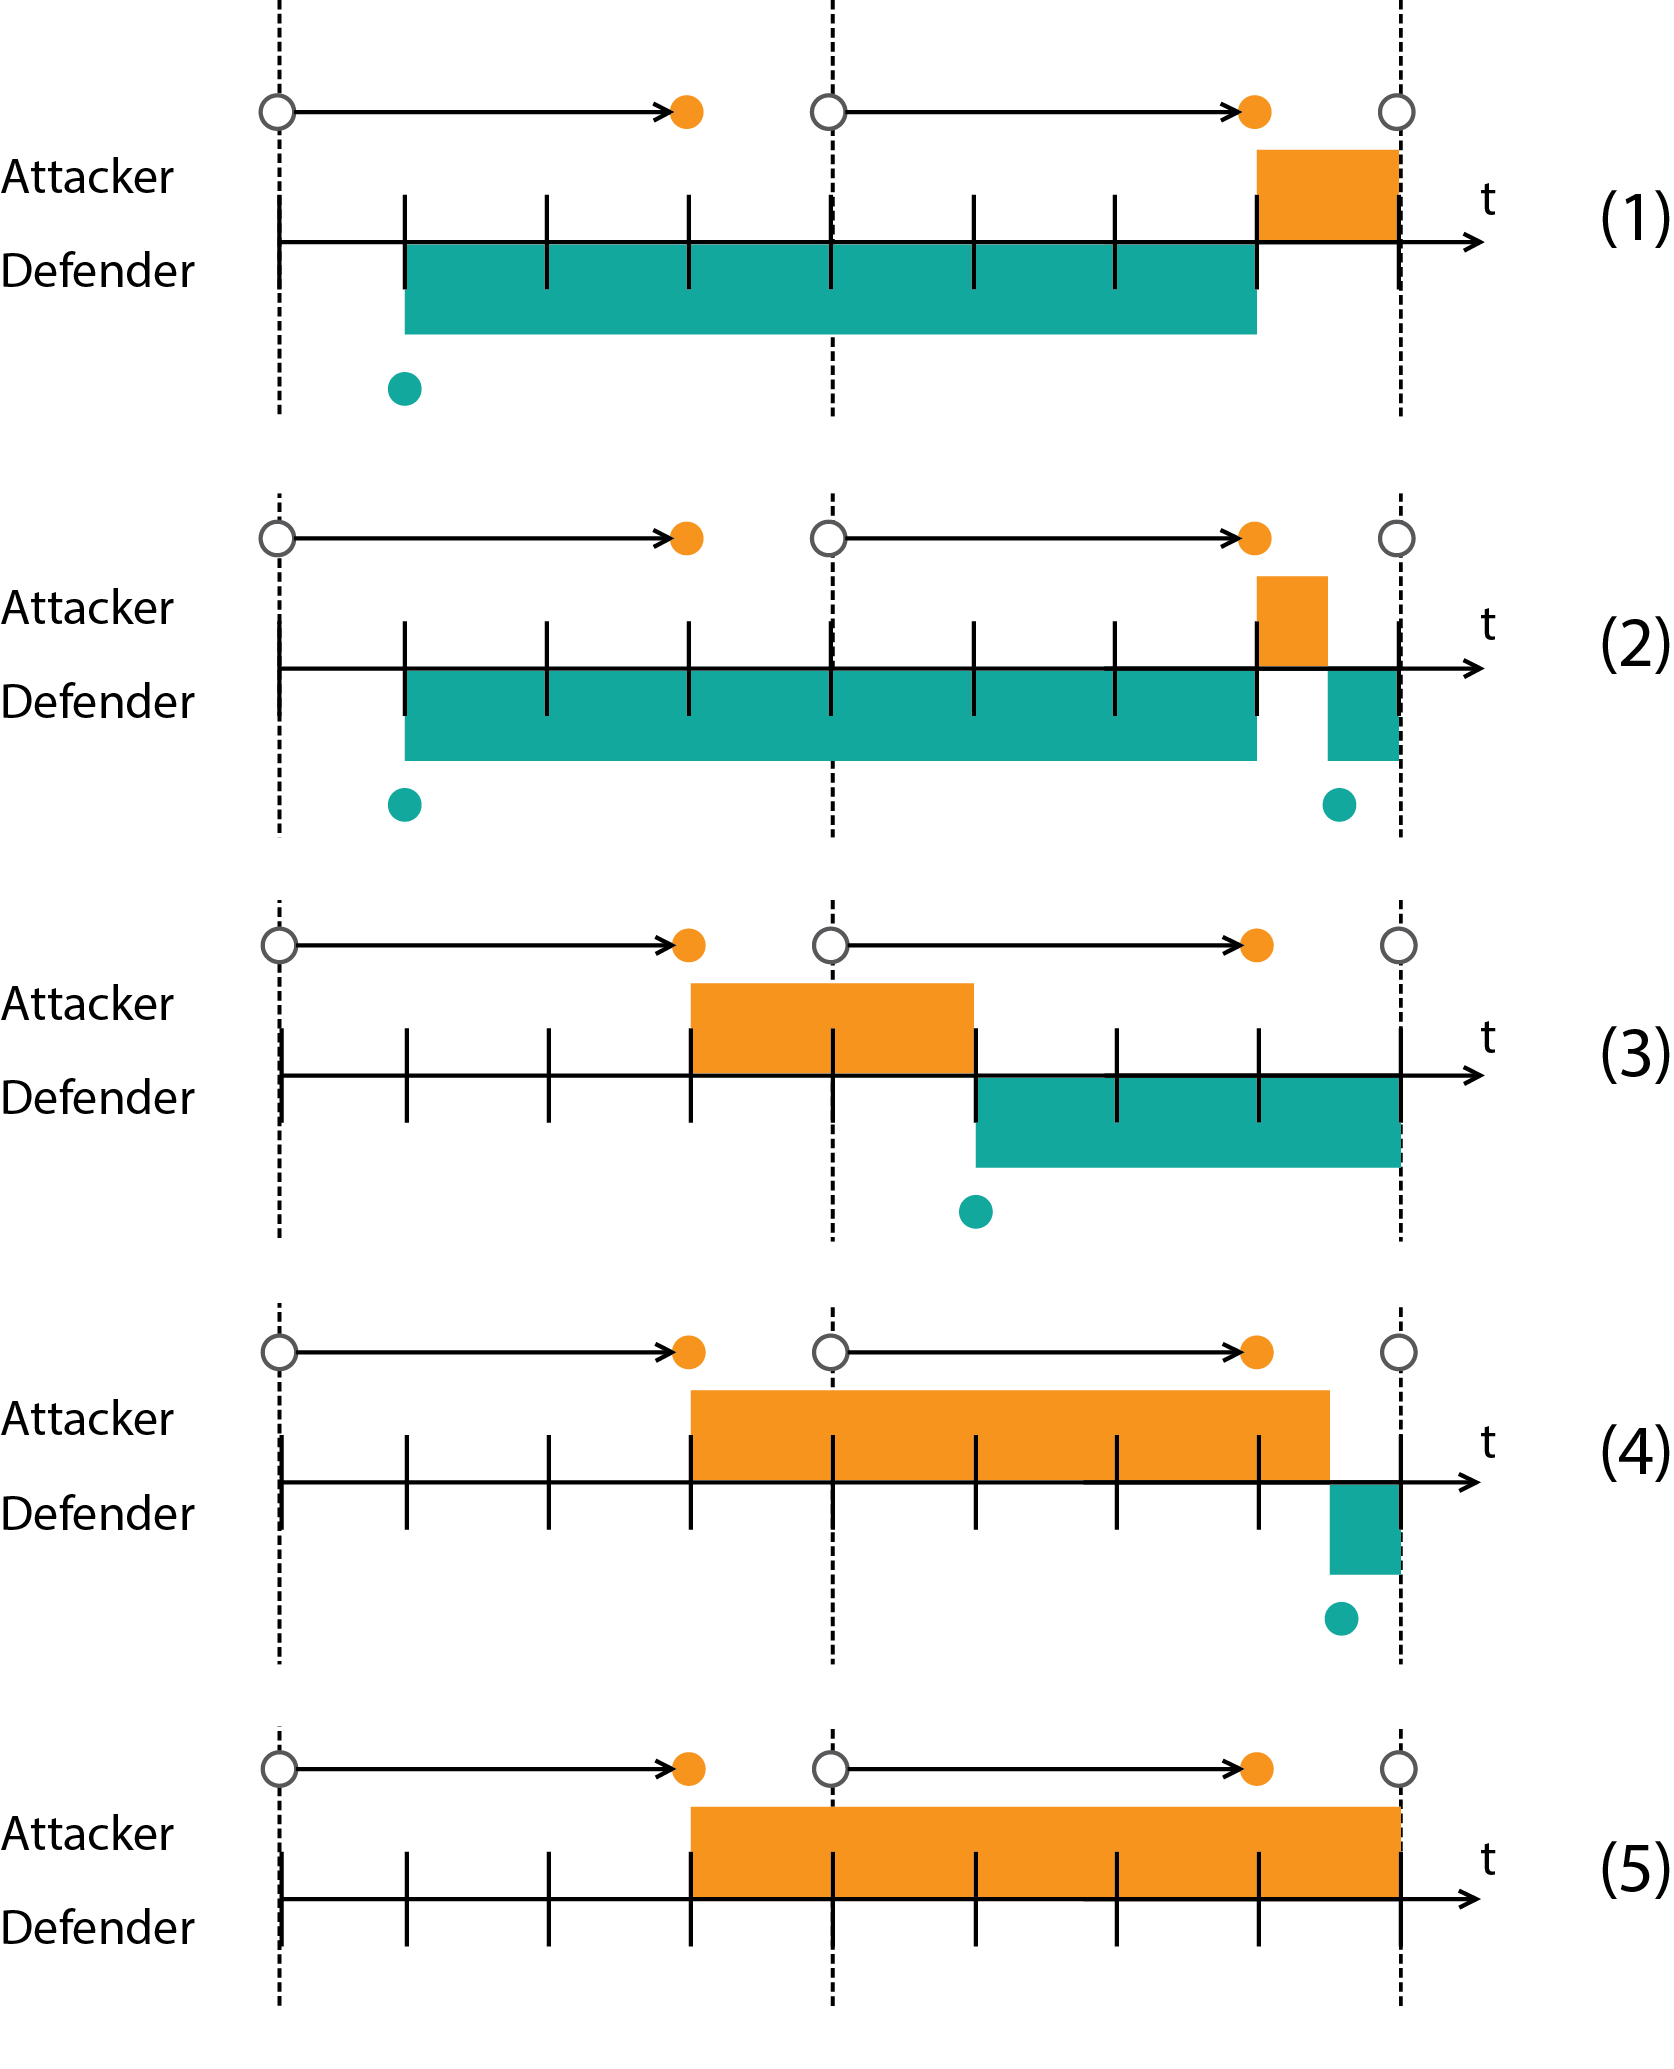
\includegraphics[scale=0.5]{../../doc/template/Images/FlipItCase2.png}
\label{fig:case2}
\end{figure}


It is crucial that $ \delta_{D}$ is at least as large as $d + \delta_{A}$. If not, this would mean that the defender can move during the delay in the interval following the interval where the defender already moved. This would mean that there can be an overlap between the average gain of $\dfrac{\delta_{A}}{2}$ and the delay. The above benefit formula would then include to much gain for the defender: the potential overlap during the delay would be counted twice. \\


~~ \\
\subsubsection*{\textbf{Case b:} $d + \delta_{A} \geq \delta_{D}$}
~~~\\

To obtain the formula in case of a too long delay, we therefore need to subtract this overlapping gain from the above formula. 
Since $\delta_{D} \geq \delta_{A}$, if the defender enters the interval immediately after the attacker has played, then the defender cannot have played in the previous interval. In that case, there is no overlap. So the problem of the overlap only appears if the defenders enters late enough and thus only the last part of the delay is subject to overlap. The larger the difference between the interval of the defender and the attacker, the smaller the risk of overlap. Concretely, only the last part of length $d - (\delta_{D} - \delta_{A})$ is subject to overlap. Hence, the probability of overlap is $\dfrac{ d - (\delta_{D} - \delta_{A})}{\delta_{D}}$ and the gain will be half of this interval:  $\dfrac{ d - (\delta_{D} - \delta_{A})}{2}$.  The gain rate to be subtracted is therefore:\\

\begin{equation}\label{first}
\dfrac{1} {\delta_{A}} \cdot \dfrac{d - (\delta_{D} - \delta_{A})}{\delta_{D}} \cdot \dfrac{d - (\delta_{D} - \delta_{A})}{\delta_{D}}
\end{equation}

The total gain  rate of the defender is obtained by subtracting this term from the gain rate of case a:
 \begin{equation}\label{first}
\gamma_{D}(\alpha_{D},\alpha_{A}) = \dfrac{\delta_{A}}{\delta_{D}} \cdot \dfrac{(d+\dfrac{\delta_{A}}{2})}{\delta_{A}} - \dfrac{(d - (\delta_{D} - \delta_{A}))^{2}}{2 \delta_{D} \delta_{A}}
\end{equation}
\begin{equation}\label{first}
\gamma_{D}(\alpha_{D},\alpha_{A}) = \dfrac{\delta_{A}}{2\delta_{D}} + \dfrac{d}{\delta_{D}} - \dfrac{(d - (\delta_{D} - \delta_{A}))^{2}}{2 \delta_{D} \delta_{A}}
\end{equation}\\
This yields in the following benefit formula:
\begin{equation}\label{first}
\beta_{D}(\alpha_{D},\alpha_{A}) = \dfrac{\delta_{A}}{2\delta_{D}} + \dfrac{d}{\delta_{D}} - k_{D} \alpha_{D} - \dfrac{(d - (\delta_{D} - \delta_{A}))^{2}}{2 \delta_{D} \delta_{A}}
\end{equation}\\
 
The benefit for the attacker will be as follows:
\begin{equation}\label{first}
\beta_{A}(\alpha_{D},\alpha_{A}) = 1 -\dfrac{\delta_{A}}{2\delta_{D}} - \dfrac{d}{\delta_{D}} - k_{A} \alpha_{A} + \dfrac{(d - (\delta_{D} - \delta_{A}))^{2}}{2 \delta_{D} \delta_{A}}
\end{equation}\\


\section{Related work on FlipIt}
\label{ch:extendedWork}

Various possible ways to extend FlipIt have already been proposed. 
Laszka et al. made a lot of additions and extensions to the original game of FlipIt. For instance Laszka et al. extended the basic FlipIt game to multiple resources. The rationale is that for compromising a system in real life, more than just one resource needs to be taken over. An example is that gaining access to deeper layers of a system may require breaking several passwords. The model is called FlipThem \cite{FlipThem}. Laszka et al. also use two ways to flip the multiple resources: the AND and the OR control model. In the AND model the attacker only controls the system if he controls all the resources of the system, whereas in the OR model the attacker only needs to compromise one resource to be in control of the entire system. \\

Another addition of Laszka et al. to the game of FlipIt \cite{MitigationCovert} 
is extending the game to also consider non-targeted attacks by non-strategic players. In this game the defender tries to maintain control over the resource that is subjected to both targeted and non-targeted attacks. Non-targeted attacks can include phishing, while targeted attacks may include threats delivered through zero day attack vulnerabilities. \\
One of the last important additions from Laszka et al. \cite{MitigationNonTargeted} is to consider a game where the moves made by the attacker are still covert but the moves made by the defender are known to the attacker. This means that the attacker can base his attacks on the defender's moves. Both the targeted and non-targeted attacks don't succeed immediately. For the targeted attack the time till it succeeds is given by an exponential distributed random variable with a known rate. The non-targeted attacks are modelled as a single attacker and the time till it succeeds is given by a Poisson process. The conclusion of this paper is that the optimal strategy for the defender is moving periodically. The difference with this paper is that the delay in this paper is dependent on the number of nodes that have to be flipped in a network. This cannot be modelled with the framework in the Laszka et al. paper because the delay is chosen as an exponential distributed random variable. Another difference is that in the case of the Laszka et al. paper, the moves of the defender are considered not stealthy and so the attacker knows when the defender plays. \\ 

Other authors used the FlipIt game to apply it on a specific scenario. To be able to use the FlipIt game, modifications where required for the FlipIt model.
One of the scenarios by Pham \cite{compromised} was to find out whether a resource was compromised or not by the attacker. This could be verified by the defender, who has an extra move "test" beside the flip move. The basic idea is to test with an extra action if the resource has been compromised or not. This move involves also an extra cost.\\

Finally researchers also have investigated the behaviour of humans playing FlipIt. A. Nochenson and Grossklags \cite{nochenson2013behavioral}  investigate how people really act when given temporal decisions. Reitter et al. \cite{reitter2013risk} extended the work of A. Nochenson and Grossklags to include various visual presentation modalities for the available feedback during the investigation.

\section{Conclusions and Further Research}
\label{ch:conclusion}
In this paper we presented an adaptation of the FlipIt game to the situation of virus propagation, such as to take the delay for network infection into account. We discerned two cases. In the case the defender plays faster than the attacker, the attacker simply looses the delay. In the case the attacker plays faster, each time the defender plays in an interval, he will gain extra time of the delay. The delay is therefore always detrimental to the benefit of the attacker. 
This demonstrates that the FlipIt game can be adapted to a game with virus propagation. Further research needs to be performed to calculate the impact of the delay on Nash equilibria and the determination of optimal defender and attacker strategies.

\bibliographystyle{IEEEtran}
\bibliography{IEEEabrv,references}

\end{document}